\documentclass[12pt]{report}

\usepackage[a4paper, total={6in, 8in}]{geometry}

\usepackage{caption}
\usepackage{float}
\usepackage{hyperref}
\usepackage{graphicx}
\usepackage[nottoc, numbib]{tocbibind}
\usepackage{outlines}
\usepackage{listings}

\begin{document}

\author{Philipp Liermann 20-475873-20\\Supervisor: Prof. Dr. Raad Bin Tareaf}
\date{\today}

\title{
\begin{center}
	
\includegraphics[width=8cm]{./images/logo.png}
\end{center}
\vspace{2cm}
Hardening MFA web applications to counter evolving transparent phishinging attack
vectors
\vspace{2cm}
\large }

\maketitle

\newpage
\tableofcontents

\newpage
\section{Problem statement}
These days most websites have implemented two or multi-factor authentication systems
to prevent malicious third-party actors from using stolen login credentials to
commit identity theft. Despite this, a new technique referred to as transparent
proxy phishing still provides malicious actors the means to bypass two-factor authentication
systems during social engineering based phishing attacks. This creates a
critical security vulnerability, as this technique can be used to gain unauthorized
access to otherwise secure systems. To resolve this issue, it is imperative to
develop and implement effective measures to counteract transparent phishing and
other methods of circumventing multi-factor authentication systems.

\section{Research question}
How can we protect multi factor authentication secured web applications from transparent
proxy phishing attacks? Based on this question the following sub questions
were derived:
\begin{itemize}
	\item What exactly are classical phishing attacks in general and how do they
	      differ from the new attack vector?

	\item How big is the threat imposed by this new type of phishing attack?

	\item Why are many organizations still not aware of this issue?

	\item What can be done to help developers counteract this type of security threat?
\end{itemize}

\section{Objective}
As credential theft and cyberfraud in general are still a growing problem in
the digital age, it is important to develop and implement effective measures to
counteract this threat. The objective of this thesis is to find and document
different strategy's that can help organizations and developers to protect their
applications against the new transparent proxy phishing attack vector.

\section{Theoretical foundations \& current state of research}
Cyberfraud is a form of internet-based fraud, usually involving the use of false
identities and/or stolen information to illegally obtain money, property, or services.
Cyberfraud is an increasingly pervasive problem that is becoming increasingly
difficult to combat, as fraudsters become more sophisticated in their methods.
In 2020, cyberfraud was estimated to cost the global economy over \$6 trillion\cite{6trillion},
with the financial sector suffering the most damages. The social, economic and
reputational costs of cyberfraud can be incredibly damaging, and can range from
the loss of money, to identity theft, to the disruption of businesses.
Cyberfraud has become so pervasive that it is essential for businesses and
individuals to take measures to protect themselves from it. This includes using
strong passwords, using two-factor authentication, and staying up to date with
the latest security protocols. \\ \\ A phishing attack is a type of
cyberattack in which an attacker attempts to gain confidential information, such
as passwords, credit card numbers, or other sensitive information, by sending
emails or other messages disguised as legitimate entities. These messages often
include malicious links to faked login prompts that will steal the victims credentials
upon entering them. These attacks are becoming increasingly sophisticated and
difficult to recognize, making it important for everyone to remain vigilant and
take steps to protect against them. \\ \\ A HTTP reverse proxy is a type of
proxy server that retrieves resources on behalf of a client from one or more
servers. This type of proxy is sometimes referred to as a “gateway” or “tunneling”
proxy because it acts as a gateway for the traffic to and from the server. A
reverse proxy will typically receive a request from a client, then forward that
request to an appropriate server on the same network. It then retrieves the
response from the server and sends it back to the client. This type of proxy server
is most often used in enterprise networks to protect against malicious traffic,
to balance load between multiple servers, and to cache static content. \\ \\
Transparent proxy phishing is a new technique used by attackers to intercept
and steal multi-factor authentication (MFA) tokens from unsuspecting users. Instead
of copying HTML code from the original page that the attacker is trying to impersonate,
this new attack uses a HTTP reverse proxy to just redirect the users traffic
to the original page. The attacking proxy operator can view and modify all traffic
that is going through it while the victim sees a one by one copy of the original
login page. By doing so login credentials and 2FA tokens can be extracted
easily. \\ \\ TLS is a cryptographic protocol that provides end-to-end security
for data sent between a client and a server. It is widely used to secure web
traffic, email, and other types of data. TLS is the successor to SSL, and is
often referred to as SSL/TLS. If a webserver is using TLS its URL starts with the
well known https:// prefix. \\ \\ TLS Fingerprinting is a technique used to identify
the TLS implementation of a client or server by analyzing the handshake process.
This can be used to identify which software is used by client or server. Industry
standards for fingerprinting algorithms have existed for a long time. These
include: JA3, JA3N and the whole JA4+ family. \\ \\
Nginx is a popular open-source web server and reverse proxy server. It is used by
millions of websites to serve web pages and other content. Nginx is known for its
high performance, stability, and low resource usage. It is also known for its
flexibility and extensibility, as it can be easily extended with third-party modules
and plugins. Because Nginx can easily be configured to act as a reverse proxy and
supports TLS, it is often used as a so called TLS terminator, meaning that it
terminates the TLS connection and forwards the unencrypted traffic to a HTTP backend
app. \\ \\
Docker is a platform for developing, shipping, and running applications. It allows
developers to package their applications and dependencies into containers, which
can then be run on any system that has Docker installed. Docker containers are
lightweight, portable, and self-sufficient, making them an ideal platform for
deploying applications. \\ \\
HTML is the standard markup language for creating web pages and web applications.
It is used to structure and present content on the web. HTML is used in conjunction
with CSS and JavaScript to create interactive and visually appealing web pages.
\\ \\
Unicode is a standard for encoding, representing, and handling text in most of the
world's writing systems. It is used to represent characters from all of the world's
writing systems, including Latin, Cyrillic, Greek, Arabic, Hebrew, Chinese, Japanese,
Korean, and many others. Unicode is used in many modern software applications,
including web browsers, word processors, and operating systems. In computer science
literature, Unicode symbols are often represented as U+ followed by a hexadecimal number. \\ \\
Many scientific papers have been published on this topic, but there is still a
lack of information on how to protect against this new attack vector. This is why
it is important to find and document different strategies that can help organizations
and developers to mitigate this new attack vector. \\ \\
Wireshark is a popular open-source network protocol analyzer that is used to capture and
analyze network traffic. It is widely used by network administrators, security
professionals, and developers to troubleshoot network problems, analyze network
traffic, and detect security vulnerabilities.

\section{Research design}
This thesis will be conducted in a quantitative research design. By analyzing
existing literature and scientific papers on the topic, but also by running own
experiments in which open source reverse proxy phishing toolkits will be used to
setup attack simulations with the goal to find flaws in their attack implementation.
With the gained knowledge from this experiments this paper will outline easy
to follow strategies to protect web services from this threat.

\newpage
\chapter{Literature Review}
\section{Overview of Multi-Factor Authentication}

Multi-Factor Authentication (MFA) is a security system that requires more than
one method of authentication from independent categories of credentials to verify
the user's identity for a login or other transaction. The most common
categories are \cite{mfa}:
\begin{itemize}
	\item Something the user knows (e.g. a password)

	\item Something the user has (e.g. a smartphone)

	\item Something the user is (e.g. a fingerprint)
\end{itemize}
MFA is used to protect the user from unauthorized access to their accounts,
and is widely used in the financial and healthcare industries, as well as in government
and military applications. MFA is also used in consumer applications, such as online
banking and e-commerce. The use of MFA is growing rapidly, as more and more organizations
recognize the need for stronger security measures to protect their users and their
data. \\ \\ MFA is a critical component of a strong security posture, and is an
essential tool for protecting against a wide range of cyber threats, including
phishing, credential theft, and identity theft. MFA is also an important tool for
protecting against insider threats, as it can help to prevent unauthorized
access to sensitive data and systems. MFA is also an important tool for protecting
against the growing threat of cyberfraud, as it can help to prevent
unauthorized access to financial accounts and other sensitive information. \\ \\

\section{Phishing Attacks: Evolution and Impact}
Phishing attacks are a type of cyberattack in which an attacker attempts to gain
confidential information, such as passwords, credit card numbers, or other
sensitive information, by sending emails or other messages disguised as legitimate
entities. These messages often include malicious links to faked login prompts
that will steal the victims credentials upon entering them. These attacks are becoming
increasingly sophisticated and difficult to recognize. Phishing has evolved
over time, from simple scams to sophisticated attacks that are difficult to detect.
In the early days of the internet, phishing attacks were relatively simple and
easy to recognize. However, as technology has advanced, so have phishing
attacks. Today, phishing attacks are often highly sophisticated and difficult
to detect, making them a significant threat to individuals and organizations.
\\ \\
Classical phishing fake login pages were usually simple HTML copies of the original
login page, but connected to a fake backend service that would store the entered credentials and
redirect the user to the original page or a fake error page. This way victims could recognize
that they had fallen for a fake login page and update their credentials before the attacker could
use them. \\ \\
The new transparent proxy phishing attack vector is a new technique used by attackers
to intercept and steal multi-factor authentication (MFA) tokens from unsuspecting
users. Instead of copying HTML code from the original page that the attacker is
trying to impersonate, this new attack uses a HTTP reverse proxy to just redirect
the users traffic to the original page. The attacking proxy operator can view and
modify all traffic that is going through it while the victim sees a one by one
copy of the original login page. By doing so login credentials and 2FA tokens
can be extracted easily. Also the victim will not recognize that he has fallen
for a phishing attack, because the website actually behaves as expected. The user
will not be redirected to a fake error page or the original page after entering
his credentials, because a real session is established with the original server. \\ \\
In summary the advantages over the classical fake HTML login page based attack are:
\begin{itemize}
 \item Knowing basic web development techniques including HTML, CSS and JavaScript
       is not required to setup a phishing attack anymore

  \item The victim will not recognize that he has fallen for a phishing attack

  \item The attacker can view and modify all traffic that is going through the proxy,
    including the entered credentials and 2FA tokens

  \item Custom HTML and JavaScript can be injected into the original page to steal even more
    information from the victim using social engineering techniques
\end{itemize}
In April 2017 a John Hopkins University Student named Xudong Zheng published a blog post with a proof of concept
on how he used a homograph attack to impersonate apple.com. He used the Cyrillic letter "a" (U+0430) instead of the
Latin letter "a" (U+0061) in the domain name. \\ This way he was able to register the domain "xn--80ak6aa92e.com"
which looks exactly like "apple.com" in the browser address bar. 
This attack was possible because the browser displayed the domain name in its punycode representation, which is
a way to represent Unicode with the limited character subset of ASCII used for internet host names.
\\ The combination of this attack with a transparent proxy phishing attack is especially dangerous, because
the URL in the address bar will look exactly like the original URL and also behave exactly like it due to usage of 
transparent proxying. It is close to impossible even for a educated user to recognize the he is being lured into a phishing attack.
Luckily the browser vendors were quick to react and implemented a fix for this issue. \\ \\
By reading literature on this topic, it becomes clear that performing a transparent proxy phishing attack is becoming
easier and easier. This is because of the increasing number of open source reverse proxy phishing toolkits that are
available on the internet. These toolkits are designed to allow read teams and cyber security researchers to set up and run transparent
proxy phishing attacks in a controlled environment. However, these toolkits can also be used by malicious actors to perform
real-world attacks. \\ The following are some of the most popular open source reverse proxy phishing toolkits:
\begin{itemize}
  \item Modlishka \cite{modlishka} is a low level HTTP reverse proxy framework that allows the attacker to intercept and modify
    all traffic that is going through it. It is written in Go and can be easily extended with custom plugins. Modlishka also provides
    a web interface to copy collected session data into an attackers browser to perform session hijacking attacks.
    It is also capable of injecting custom HTML and JavaScript into the original page to steal even more information from the victim.

  \item Evilginx2 \cite{evilginx2} is a more advanced transparent phishing toolkit that is also written in Go. It provides same
    capabilities as Modlishka, but also includes ready to use templates and a custom DNS server. Its more user friendly and easier to use
    than Modlishka, but also less flexible and extensible.

  \item Murena \cite{murena} is a transparent phishing toolkit that is written in Python. It is not as advanced as Modlishka and Evilginx2,
    but is still capable of intercepting and modifying all traffic that is going through it. It is also capable of injecting custom HTML and
    JavaScript into the original page.
\end{itemize}


\section{Existing Countermeasures}
The paper "Catching Transparent Phish: Analyzing and Detecting MITM Phishing Toolkits" \cite{kondracki2021catching} provides a detailed
analysis of the most used reverse proxy phishing toolkit and its potential to
bypass MFA systems. The authors demonstrate how those toolkits can be used to intercept
and steal MFA tokens, and propose a detection method based on a statistical
model that evaluates a combination of TLS fingerprinting and response timing
analysis. The authors provide an AI based solution for finding transparent phishing
toolkits in the wild, but only provide limited advice on how to detect client
connections of those toolkits on the recieving server side.

\newpage
\chapter{Experimentation}
\section{Simulation of Transparent Phishing Attacks}
To test and analyze the capabilities of the most popular open source transparent phishing toolkits
a controlled lab environment will be set up. The goal is to find flaws in their attack implementation
and to develop and test new or improved countermeasures against these attacks.
First a web application will be set up that is secured with a multi-factor authentication system.
Then the open source transparent phishing toolkits will be used to set up attack simulations against
this web application. The local web application will be running on a local machine, but still be secured
with a valid self-signed TLS certificate. Our own certificate authority will have to be installed in the
browser used for testing, a recent version of google chrome in this case. In a real world scenario an attacker
would also have to buy a valid domain name. For our simulated attacks an entry in the hosts fill be sufficient
to redirect the traffic to the local machine.

\begin{figure}[!htb]
  \centering
  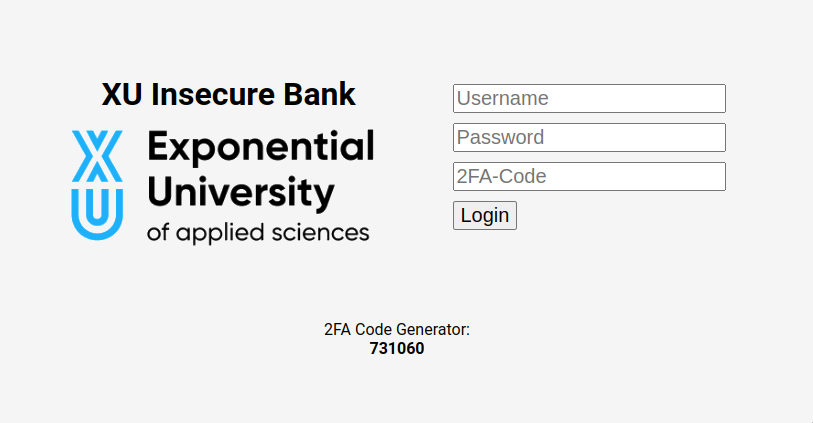
\includegraphics[height=7cm]{./images/2fa_app.png}
  \caption{Web application secured with a demo two-factor authentication system}
\end{figure}

The test environment web application implements a very basic credential based login system with two-factor
authentication. For demo purposes the two-factor authentication logic will accept any 6 digit number as
valid token.\\The frontend of this application is connected to a NodeJS based backend that is using express.js
for routing and parsing of incoming requests. After one provides login credentials in the frontend a authentication
endpoint in the backend will be called with the provided credentials. If the credentials are valid the backend
will redirect the user to his profile page. This response will also contain a session cookie that will be used
to authenticate the user in the future.\\For an attacker, stealing the content of that session cookie is enough to
gain full access to that account. This is also true for most real world web applications where cookie based authenticaion
is used, but this alone is not a securiy issue. Nearly 99\% of all websites are TLS secured today \cite{tlsPercentage} meaning
that no one except the user and server can see the content of that HTTP request including the session cookie.\\ \\

In our simulated attack scenario it will be our goal to steal the content of this session cookie to overtake the victims
session. In the real world an attacker is likely saving login credentials eg. email and password from all requests he intercepts
with his transparent phsihing toolkit's mitm proxy. Additionally he may inject custom HTML and JavaScript into the original page
to steal even more information from the victim using social engineering techniques, for example by asking for an additional
multi factor authentication token that he can use in the future. For the purpose of this experiment we will only focus on
stealing the session cookie.\\ \\

\begin{figure}[!htb]
  \centering
  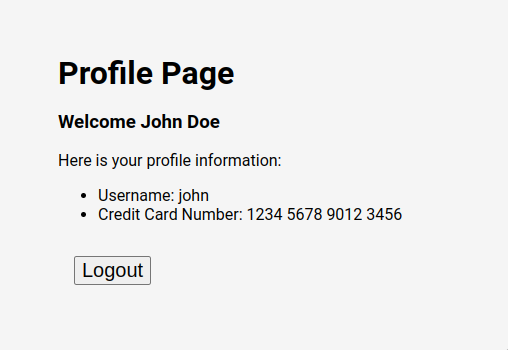
\includegraphics[height=7cm]{./images/profile_page.png}
  \caption{Profile page containing confidential information}
\end{figure}

\newpage
\section{Testing of Countermeasures}
\subsection{Blacklisting well known TLS Fingerprints}
The first countermeasure that we are trying to implement in our web applications backend is to blacklist TLS fingerprints of well known transparent phishing toolkits. This way we can detect if a client connection is relayed through a transparent phishing toolkit and show the user a warning or ignore the whole request. This approach comes with some obvious downsides:

\begin{itemize}
  \item The attacker can change the TLS fingerprint of his transparent phishing toolkit by modifying the TLS stack of the toolkit or by using a different toolkit with an unknown fingerprint
  \item The attacker can spoof the TLS fingerprint of the victim's client
  \item The attacker downgrades to HTTP and does not use TLS at all
\end{itemize}

Example implementation of a basic blocklist implemented using a custom nginx fork that supports JA4 fingerprinting:

\begin{lstlisting}
server {
    listen 443 ssl;
    server_name xu-bank.com;

    # ... other ssl configuration

    # blocklist
    map $http_ssl_ja4 $allowed_client {
      default                                 1;
      "t13d191000_9dc949149365_e7c285222651"  0; # evilginx2
    }

    location / {
        # block the request if the clients fingerprint is on the blocklist
        if($allowed_client = 0) {
            return 403;
        }

        # forward the request to the backend
        proxy_pass http://backend;
    }
}
\end{lstlisting}

The same approach can be turned into a whitelist by inverting the logic. This way only clients with a known good TLS fingerprint will be allowed to access the web application. This approach is more secure, but also comes with the downside that new clients will not be able to access the web application until their TLS fingerprint is added to the whitelist. Maintaining a trusted JA4 fingerprint database would require a lot of fingerprint collecting before said whitelist can be used in production as many different browsers and TLS implementations exist and change frequently.

\subsection{Evaluating TLS Fingerprinting Algorithms}
In general performing TLS fingerprinting on a client connection works by analyzing the TLS ClientHello message that is sent by the client to the server during the TLS handshake process. This message contains a lot of information about the client's TLS implementation, including the version of the TLS protocol that the client supports, the list of supported cipher suites and extensions. To generate a unique fingerprint out of this information several algorithms already exist. The JA3 algorithm proposed first by Salesforce \cite{ja3Salesforce} collects values from the ClientHello into four different array lists and formats them into one comma separated string that gets hashed. In detail the values used from ClientHello are: SSLVersion, Cipher, SSLExtension, EllipticCurve, EllipticCurvePointFormat. An example derived from a ClientHello looks like this: "769,47-53-5-10-49161-49162-49171-49172-50-56-19-4,0-10-11,23-24-25,0". If no SSL extensions are used the field will be left empty. Example: "769,4-5-10-9-100-98-3-6-19-18-99,,,". Generating a MD5 hash from that string will leave us with the following 32 characters: "ada70206e40642a3e4461f35503241d5". JA3 also needs to ignore values for non existing extensions, because some TLS clients are using Google’s GREASE (Generate Random Extensions And Sustain Extensibility). This is a feature proposed by Google to break wrongly implemented TLS servers. It may sound controversial at first, but comes with good intentions. In a internet draft paper by D. Benjamin \cite{greaseDraft} he explains that its better to break some production systems in place instead of risking flawed TLS implementations to spread and risk outages of global scale.\\JA3 seems to be a good candidate for fingerprinting transparent phishing toolkits at first, but it after some testing it comes clear that JA3 can not be used to fingerprint instances of Google Chrome, due to it's reliance on the order of the cipher extension list in the ClientHello package. Google chrome uses a feature called "TLS ClientHello extension permutation" that prevents TLS fingerprinting for said reason. This can be bypassed by sorting the numeric values by size. Open source implementations of the JA3 algorithm with normalized extension orders exist under the name "JA3N". Sadly in our experimentation we were not able to reliably identify versions of Google Chrome using JA3 for yet unkown reasons.\\ \\
Luckily a better alternative to the JA3 algorithm exists. The JA4+ family is a set of new network fingerprinting algorithms developed by FoxIO \cite{foxIOJa4}.
The JA4+ family also comes with a fingerprinting algorithm for TLS called JA4. JA4 is superior to JA3 in many ways. It supports HTTP 3 including its UDP based transport protocol QUIC and normalized the order of ciphers and extensions by default. It uses a different output format than JA3 which consists of three seperatable parts that more verbose and human readable in general. JA4 provides a more reliant and expressive fingerprinting solution for this papers use case. Other open-source implementations of JA4 are avaible and include a wireshark addon and an nginx fork. The later one will be used in our lab setup to collect JA4 fingerprints.

\begin{figure}[!htb]
  \centering
  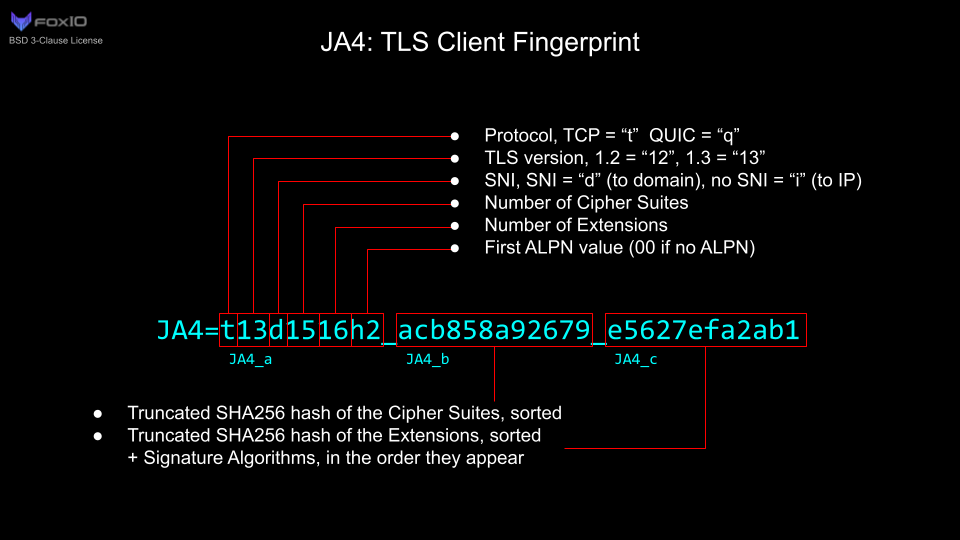
\includegraphics[height=7cm]{./images/JA4.png}
  \caption{JA4 TLS client fingerprint format}
\end{figure}

TODO: the google feature is "to reduce potential ecosystem brittleness" and not for privacy. Quote more from:
https://chromestatus.com/feature/5124606246518784

\chapter{Results}
\section{Findings from Simulations}
Present the data collected from the simulations, providing analysis and interpretation.

\section{Effectiveness of Current Defenses}
Assess the effectiveness of existing defenses against reverse proxy phishing based
on your findings.

\section{Proposed Solutions}
Introduce any new solutions or improvements to existing solutions developed through
your research.

\chapter{Discussion}
\section{Implications of Findings}
Discuss the broader implications of your findings for cybersecurity practices and
MFA implementation.

\section{Limitations and Future Research}
Acknowledge any limitations of your study and propose areas for future research.

\newpage
\bibliographystyle{plain}
\bibliography{refs}

\end{document}
